\section{\LaTeX formats}

\lipsum[1]

In \Cref{eqn:sample}, in \Cref{thm:sample}, \Cref{cor:sample}, in \Cref{lem:sample}, in \Cref{tab:sample}, in \Cref{fig:sample-1,fig:sample-2}, in \Crefrange{fig:sample-1}{fig:sample-3} in \Cref{alg:sample}.

In \cite{Abril07} and \cite{Cohen07}, but mostly in \cite{Abril07,Cohen07}.
\begin{equation}
E=mc^{2}
\label{eqn:sample}
\end{equation}


\begin{description}
	\item[Identify] Characteristics of an object.
	\item[Locate] Absolute or relative position.
	\item[Distinguish] Recognize as the same or different.
\end{description}


\begin{enumerate}
	\item Visual and auditory feedback (V\,$+$\,A).
	\item Visual feedback, no auditory feedback (V).
	\item Auditory feedback, no visual feedback (A).
\end{enumerate}


\begin{itemize}
	\item \textit{when} $+$ \textit{where} $\Rightarrow$
	\textit{what}: State the properties of an object or objects at a
	certain ~time, or set of times,  and a certain place, or set of places.
	\item \textit{when} $+$ \textit{what} $\Rightarrow$
	\textit{where}: State the location or set of locations.
	\item \textit{where} $+$ \textit{what} $\Rightarrow$
	\textit{when}: State the time or set of times.
\end{itemize}


\begin{table}[t]
\tbl{Insert table title here}{%
\begin{tabular}{|l|p{8pc}|p{8pc}|p{12pc}|}
\hline
A & \multicolumn{3}{l|}{{B}} \\\hline
{C} & {D} & \multicolumn{2}{|{c}|}{E} \\\cline{3-4}
          &  & F & G \\\hline
H & I & J & K \\\hline
L & M & N & O \\\hline
\end{tabular}}
\begin{tabnote}
Insert here your table note
\end{tabnote}
\label{tab:sample}
\end{table}


\begin{quote}
\lipsum[1]
\end{quote}

\begin{theorem}[Theorem Name]
	\label{thm:sample}
	\lipsum[1]
	\begin{proof}
		\lipsum[1]
	\end{proof}
\end{theorem}

\begin{corollary}
	\label[cor]{cor:sample}
	\lipsum[1]
\end{corollary}

\begin{lemma}
	\label[lem]{lem:sample}
	\lipsum[1]
\end{lemma}


\begin{figure}[tp]
	\centering
	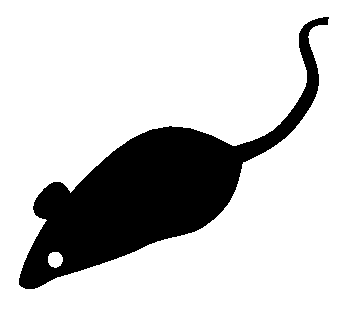
\includegraphics{./fig/acmlarge-mouse}
	\caption{Insert here your figure caption.}
		\label{fig:sample-1}
\end{figure}


\begin{figure}[tp]
	\begin{minipage}[t]{0.45\linewidth}
		\centering
		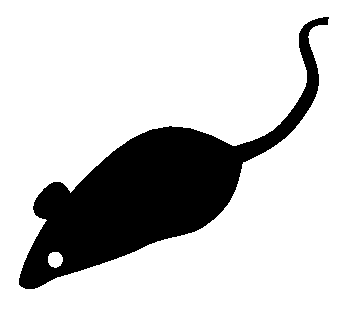
\includegraphics{./fig/acmlarge-mouse}
		\caption{Insert here your figure caption.}
		\label{fig:sample-2}
	\end{minipage}
	\hspace{0.1\linewidth}
	\begin{minipage}[t]{0.45\linewidth}
		\centering
		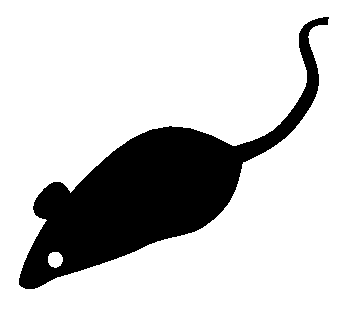
\includegraphics{./fig/acmlarge-mouse}
		\caption{Insert here your figure caption.}
		\label{fig:sample-3}
	\end{minipage}
\end{figure}


\medskip
\begin{algorithm}[H]
	\SetAlgoNoLine
	$variable \leftarrow$ value \\
	$variable$ is inside circle \\
	\While{$variable$ is inside circle,}{
		$neighborhood \leftarrow$ all grid hexes within two hexes from $current\_position$ \\
		\For{ each $hex$ in $neighborhood$, }{
			\For{each $neuron$ in $hex$}{
				convert $neuron\_orientation$ to $vector$ \\
				scale $vector$ by $neuron\_excitation$ \\
				$vector\_sum \leftarrow vector\_sum + vector$
				}
			}				
			normalize $vector\_sum$ \\
			return $current\_position$ \\
	}
	\caption{Insert here the title of your algorithm}
	\label[alg]{alg:sample}
\end{algorithm}
\medskip
				